\section{User Based Evaluation}
Following the expert evaluation, we have addressed the majority of the usability problems. It is now time to return to the users for an evaluation based on their feedback. We will conduct an evaluation involving the target users of the system. User-based evaluation techniques include various methods, each with its advantages and disadvantages. The most commonly used techniques are Think Aloud and Controlled Experiments. Therefore, we have decided to implement both.
	\subsection{Think Aloud}
	The Think Aloud method is based on simple principles. We gathered a group of seven people, presented them with our prototype, and conducted the experiment using the following criteria:
	\begin{enumerate}
		\item We introduced ourselves, explained the purpose of our application, and outlined the goals of our evaluation.
		\item Each participant was asked to individually complete the same task: add a document and then edit it.
		\item We clarified that we were testing the application’s design, user-friendliness, and usability, not the participants themselves.
		\item The experiment took place in person, with each participant using Prototype One of Expire Guard.
		\item During the tasks, we asked participants to explain their actions, thoughts, and any doubts they had out loud.
		\item We took notes with pen and paper, which were later refined in Microsoft Word.
	\end{enumerate}
	\noindent
	We chose these tasks because they represent the main functionalities of our application. The participants included university students and adults with varying levels of experience with smartphones and mobile applications, all fitting the age range identified in our user requirements.\\
	The results were very positive:
	\begin{itemize}
		\item Participants found the user interface easy and intuitive.
		\item They easily located the 'add document' feature and navigated the adding wizard without issues.
		\item They then proceeded to the document's detail page, edited the document, and saved it without hesitation.
	\end{itemize}
	\noindent
	None of the participants encountered problems completing the tasks, indicating that the graphical interface effectively guided users without causing misunderstandings or confusion.
	\clearpage
	\noindent
	Given the positive outcomes, we asked participants for feedback on their experience and any potential improvements. One participant made a suggestion: when adding a document via camera scan, he preferred to scan the document first and then fill out the form, rather than the sequence in the prototype.\\
	Another group of participants suggested removing the "folder" button located in the lower left center of the screen. While the button's purpose was clear, they felt it was unnecessary since users could easily return to the homepage from any part of the application without it. Removing this button could also give the "+" button more emphasis, making it stand out even more.	
	
	
	
	
	
	
	
	\subsection{Controlled Experiment}
	A controlled experiment is a method where the environment under test is kept constant, except for one variable. Typically, a state of the system is designated as the control group, usually representing the normal or standard condition. Another group, the experimental group, is then compared to this control group. All conditions between these two groups are identical except for the one variable being tested.\newline
	In a controlled experiment, every aspect of the environment is maintained to ensure that only the variable being examined can change. This allows researchers to measure the specific effects of that variable accurately. The goal is to isolate the variable's impact, providing clear and measurable data on how it influences the outcome.\newline
	Controlled experiments are considered the most rigorous empirical methods available. They provide strong evidence to support or refute a particular claim or hypothesis, as they minimize the influence of external factors and focus solely on the variable in question.By maintaining strict control over experimental conditions, controlled experiments ensure that the results are attributable to the variable being tested, making them a powerful tool in empirical research.
		\subsubsection{First experiment}
		We used this tool to help us decide between two different solutions for our graphical interface. Specifically, we examined the alternatives shown below. In the first option, we used an icon to represent the button that allows users to go back to the previous page. In the second option, we used a hyperlink with the text “Go back to resume page.” These two alternatives serve as our independent variables in this comparison.\newline
		By evaluating these two design choices, we aimed to determine which one provides a better user experience. The icon-based button offers a visual cue that is often quickly recognized by users, while the text-based hyperlink provides a clear and direct instruction. Our goal was to see which approach users found more intuitive and efficient for navigation.
			\begin{figure}[htbp]
				\centering
				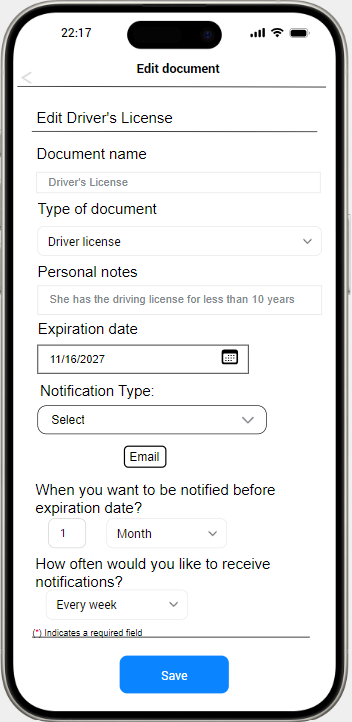
\includegraphics[width=0.4\textwidth]{../mockups/edit_variant.png}  % Replace 'example-image' with the filename of your image
				\caption{Original version, called "icon"}
			\end{figure}
			\clearpage
			\begin{figure}[htbp]
				\centering
				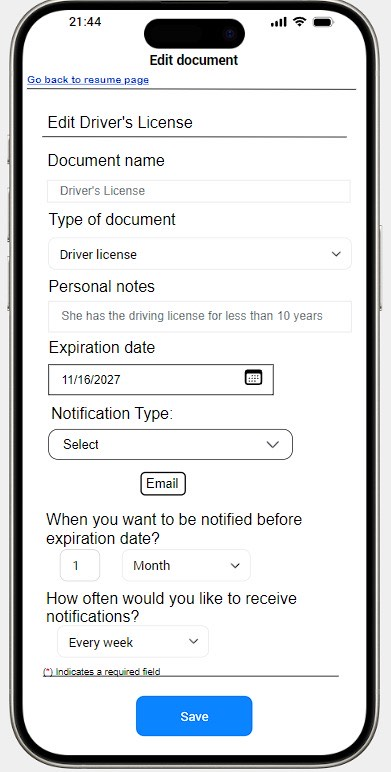
\includegraphics[width=0.4\textwidth]{../mockups/go_back_variant.jpg}  % Replace 'example-image' with the filename of your image
				\caption{Alternative version, call "text"}
			\end{figure}
			\noindent
			With our experiment underway, we defined the following hypothesis: users will make fewer errors with the version shown in Figure 23 compared to the alternative version in Figure 24. As is standard practice, we also established the null hypothesis: there will be no significant difference between the two versions in terms of errors made. The dependent variable we measured was the number of errors participants made while completing the task of editing a document.\newline		
			We recruited a total of eight participants within the user range specified in previous sections. Each participant was tasked with editing a document, and we employed a within-group method, meaning every participant tested both versions of the interface. This approach helped eliminate bias and reduced the number of participants needed. However, it also introduced the possibility of transfer of learning, where experience with the first version could influence performance on the second.\newline
			To mitigate this factor, we had four participants start with the first version and then switch to the second, while the other four participants started with the second version and then switched to the first. This counterbalancing method helped reduce the impact of learning transfer, ensuring that our results were more reliable and reflective of the true differences between the two interface versions.\\
			\clearpage
		\subsubsection{ANOVA}
			Following the experiment, we obtained eight values representing the errors made by participants for each version.To interpret the results, we will conduct a statistical analysis aimed at disproving the null hypothesis and identifying the optimal version. We employed ANOVA (Analysis of Variance) for this purpose, a statistical method that evaluates variance using the F-test. This analysis can be conveniently performed using Microsoft Excel.\\
			\begin{figure}[htbp]
				\centering
				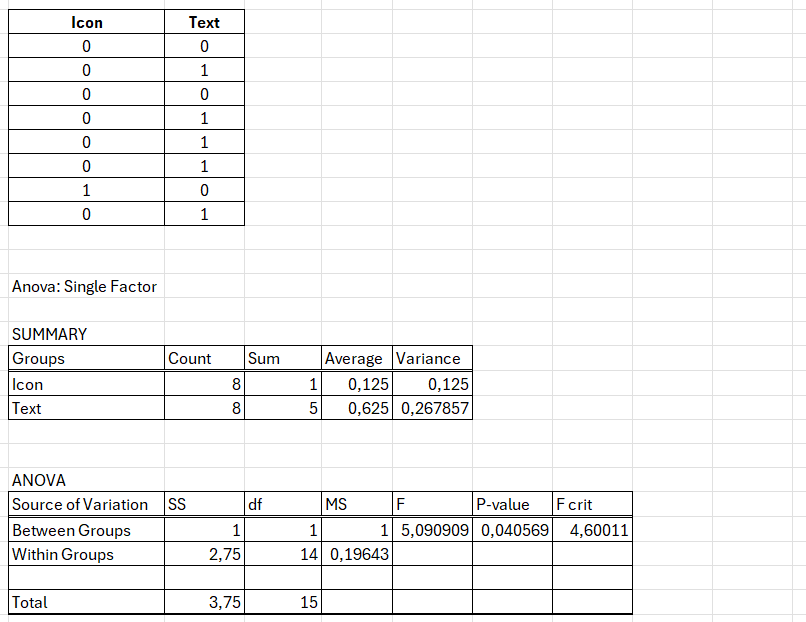
\includegraphics[width=1\textwidth]{../Draw.io diagrams/anova_icon_text_better.png}  % Replace 'example-image' with the filename of your image
				\caption{Anova computation of the first experiment}
			\end{figure}
			
			\noindent
			Since our analysis showed \textit{F} \(>\) \textit{F crit}, we can reject the null hypothesis and use this evidence to support the conclusion that the first alternative is more intuitive than the second. This result is likely due to the icon being commonly associated with returning to a previous page without completing the current task. In contrast, the hyperlink text may cause confusion, especially among users in the older age group or those less familiar with smartphones and mobile applications.\\ When these users see the hyperlink text in the upper left corner upon opening the page, they might mistakenly believe it is where they should click after completing the task, such as editing the document in this case.
			\clearpage
		\subsubsection{Second experiment}
			Our second experiment aimed to determine whether we could create a better and more intuitive version of the main page of our application. Specifically, we investigated whether adding text to the button for the "Add Document" feature would enhance our design. These two alternatives will serve as independent variables in this comparison.
			\begin{figure}[htbp]
				\centering
				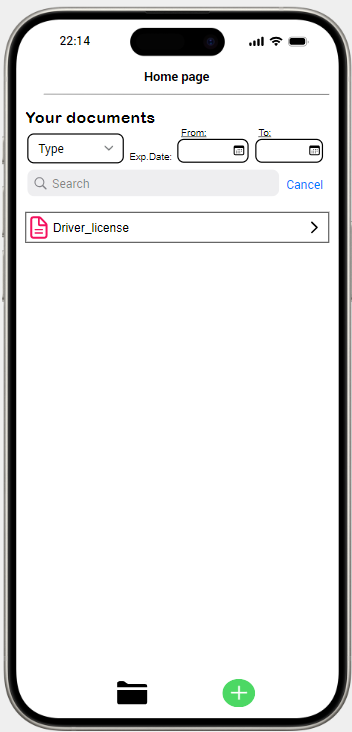
\includegraphics[width=0.4\textwidth]{../mockups/plus_variant.png}  % Replace 'example-image' with the filename of your image
				\caption{Original version, called "+"}
			\end{figure}
			\clearpage
			\begin{figure}[htbp]
				\centering
				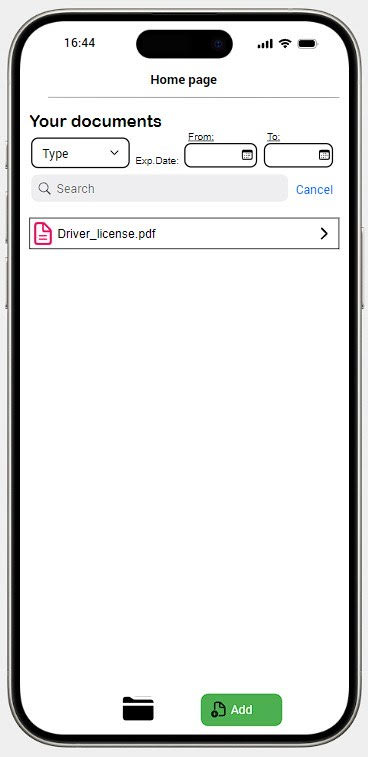
\includegraphics[width=0.4\textwidth]{../mockups/add_variant.jpg}  % Replace 'example-image' with the filename of your image
				\caption{Alternative version, call "add"}
			\end{figure}
			\noindent
			We now define the following hypothesis: the version shown in Figure 26 will lead users to operate more quickly than the alternative version shown in Figure 27. As usual, we also define the null hypothesis: there will be no speed difference between the two versions. In this case, the dependent variable we measure is the time taken by subjects to complete the task of adding a document. The experiment is conducted under the same conditions as the first experiment.\\
			\clearpage
		\subsubsection{ANOVA}
			In this case, we obtained a series of eight time values (measured in seconds and rounded up to the nearest integer) for each version. As previously mentioned, we will now conduct our analysis using the ANOVA statistical technique.
			\begin{figure}[htbp]
				\centering
				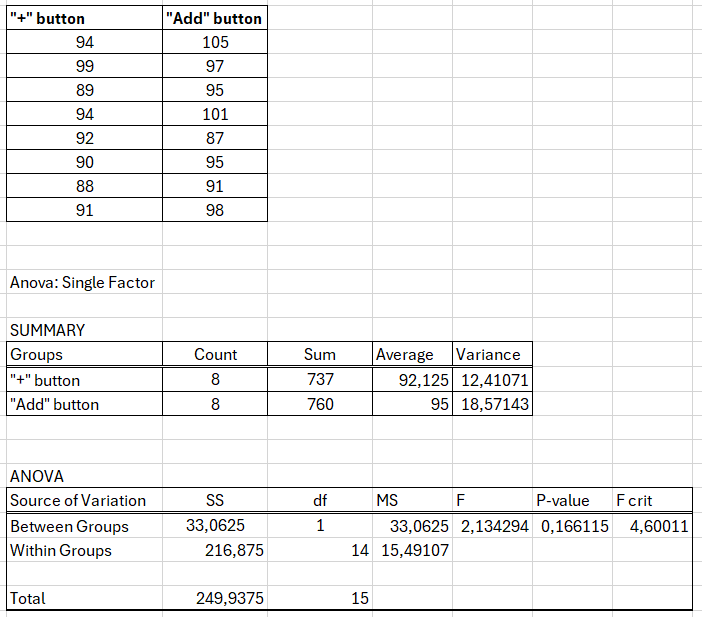
\includegraphics[width=1\textwidth]{../Draw.io diagrams/anova_+_add.png}  % Replace 'example-image' with the filename of your image
				\caption{Anova computation of the first experiment}
			\end{figure}
			
			\noindent
			The statistical analysis of the second experiment resulted in \textit{F} \(<\) \textit{F crit} indicating that we must reject our hypothesis and accept the null hypothesis. This suggests that changing the button to the alternative version will not improve our design. This is likely because the "add document" feature, being the main function of the application, is already sufficiently highlighted and easy to understand in the current design we developed.
			\clearpage
\subsection{Gatherings}
At the end of the User-Based Evaluation, we confirmed that the steps taken following the Expert Evaluation were effective. There were no issues during this phase, and the general satisfaction of the users demonstrated that the interface design is both easy and intuitive for new users while efficiently supporting the tasks it needs to accomplish. It provides all the necessary tools for users to set custom reminders for document expiration dates.\\
We decided not to follow the suggestion from the user to change the order of the pages in the "add document with camera scan" feature, as this feedback was unique to a single participant. All other users found the existing design to be optimal.
After thorough consideration, we accepted the other suggestions from participants in the Think Aloud sessions. Specifically, we decided to remove the 'folder' button from the design. The reasons provided were valid, and after verifying that the application would remain equally functional without the button, we concluded that its removal was beneficial.
